
\chapter{Arquitetura do Protótipo}
\label{cha:arquitetura}

Neste capítulo é apresentada a arquitetura definida para concretizar o protótipo.

\section{Desenho} 
\label{sec:arquitetura}

Nesta secção está detalhado o desenho do sistema.

\begin{figure}[ht]
	\centering
	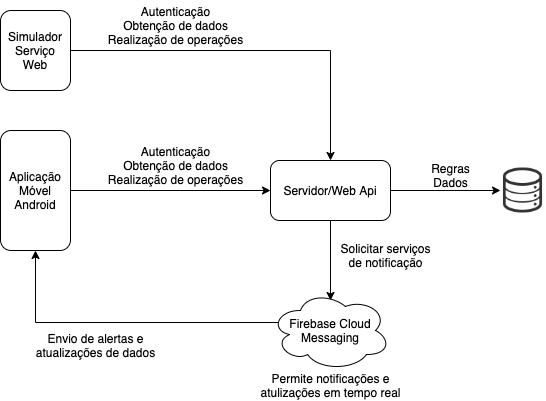
\includegraphics[width=0.85\textwidth]{arq}
	  \caption{Arquitetura do sistema}
  \label{fig:arq_s}
\end{figure}


\subsection{Componentes do Sistema} 
\label{sec:arquitetura}

O sistema, ilustrado na \figurename~\ref{fig:arq_s}, é constituído pelas seguintes componentes:
\begin{itemize}
\item Aplicação móvel
\item Servidor/Web \acrshort{api}
\item Firebase Cloud Messaging \cite{firebase}
\item Simulador de Serviço
\end{itemize}

A \textbf{aplicação móvel}, implementada em Android, corresponde à componente que define a aplicação cliente do sistema. Esta componente é responsável por fornecer uma interface gráfica de suporte às funcionalidades disponibilizadas pelo sistema. De forma a receber atualizações em tempo real e notificações a aplicação utiliza a API do \textit{Firebase Cloud Messaging}.

A componente \textbf{Servidor/Web \acrshort{api}} é a responsável pela gestão das senhas do sistema. Ela define as operações que permite aos utilizadores a observação e obtenção de senhas de interesse.
O acesso às operações suportadas é realizada por meio da \acrshort{api} disponibilizada pelo servidor. O envio de notificações e de atualizações em tempo real é realizado através da interação com os servidores \textit{Firebase Cloud Messaging}. Por estar numa fase de prototipagem, esta componente gere de forma direta a autenticação de utilizadores no sistema. Para persistência de dados, é utilizada uma base de dados PostgreSQL.

\textbf{\acrfull{fcm}}, é uma solução \textit{cross-platform} em nuvem, que fornece ao sistema soluções/serviços que permitem enviar mensagens e notificações de forma confiável às componentes clientes do sistema. A plataforma \textbf{Firebase} disponibiliza toda a infraestrutura para oferecer o serviço.
Para delegar o \textit{push} de mensagens e notificações às componentes cliente é utilizado o protocolo HTTP.

O \textbf{Simulador de serviço}, concretizado em Flutter, corresponde à componente que faz a simulação daquilo que acontece nos postos de serviço, no que diz respeito à mudança de estados das filas e permite a gestão dos serviços, postos de serviços e as filas, funcionando como um \textit{backoffice}.

Cada seta apresentada na \figurename~\ref{fig:arq_s}, representa o fluxo/interação entre cada componente do sistema.

\subsection{Interação entre Componentes}
\label{sec:arquitetura}
Existem várias interações entre as componentes do sistema, por forma a capacitar a disponibilização das funcionalidades desenvolvidas.

O sistema utiliza o modelo \textbf{cliente-servidor}, com o servidor responsável pela disponibilização de uma \acrshort{api} que permite ao cliente a realização de operações. Este serviço, em conjunto com a aplicação cliente móvel ou simulador de serviço, disponibiliza ao utilizador uma interface gráfica, que permite a realização das operações e acesso a recursos.

Por forma a permitir a apresentação do estado das filas de determinados serviços e anunciar ao utilizador que a sua vez de ser atendido se aproxima, é utilizado o mecanismo de notificações em tempo real, com base no modelo \textit{push notifications} \cite{observerpattern}. Para capacitar ao sistema com este recurso, utiliza-se a componente {\acrshort{fcm} como serviço externo. A interação das componentes funciona com o padrão de \textit{publish-subscribe} \cite{publishsubscribe}, em que o utilizador através da aplicação, subscreve a atualizações de forma explícita, ou seja, quando obtém uma senha de um serviço, e de forma implícita, ao entrar num ecrã que apresenta os estados das filas em que tem interesse. Ao sair do ecrã ou da aplicação a subscrição é retirada. O servidor é a componente que tem a informação sobre as subscrições efetuadas, realizando o envio de notificações/mensagens, recorrendo ao serviço externo \acrshort{fcm}. O envio é realizado quando existe o desencadeamento de eventos de interesse dos utilizadores.

\section{Implementação} 
\label{sec:implementacao}
Nesta secção é detalhada a implementação dos componentes que permitem o funcionamento do sistema.

O código fonte do sistema está presente no repositório: \\ \url{https://github.com/Pompeu208/isel-tfm-sgpfe-rn.git}.

\subsection{Componentes} 

O transporte de dados entre componentes, é feito utilizando o formato \textbf{\textit{hypermedia Siren \cite{siren}}}, que permite a utilização de \textit{link relations} e \textit{actions}. Com este formato, a componente cliente não precisa de saber \textit{à priori} todas as operações permitidas pelo sistema, recebendo nas respostas da \acrshort{api} que tipos de ações é que se pode realizar sobre determinado recurso.

A \textbf{\acrfull{api}} disponibilizada pelo servidor, que define as operações existentes no sistema e faz a gestão das senhas foi desenvolvida utilizando a \textit{framework} \textbf{\textit{Spring Boot}}, com \textbf{\textit{Kotlin}} a ser utilizado como linguagem de programação. \textbf{\textit{Spring Boot}} apenas facilita a configuração \textit{Spring}, sendo \textbf{\textit{Spring MVC}} \cite{springmvc} a \textit{framework} que oferece a arquitetura utilizada no servidor, \textit{\acrfull{mvc}} \cite{mvc}.
A componente, de forma a receber pedidos externos, utiliza o conceito de \textbf{\textit{Controller}}, para a definição dos \textit{handlers} para cada recurso do sistema. Com este conceito, foram desenvolvidos \textit{controllers} relacionados com o recurso utilizador e senha, de forma a permitir a entrada no sistema de forma segura, e permitindo aos utilizadores e serviços externos realizarem operações que permitem a gestão das senhas disponibilizadas pelos postos dos serviços. 
É utilizado o conceito de \textbf{\textit{Services}}, de forma a definir as interfaces e respetivas implementações que permitem ter uma camada com a lógica de negócio. De forma a aceder aos dados presentes nas entidades do modelo físico, é implementado em Spring uma camada de acesso a dados (\acrshort{dal}). A camada de acesso a dados foi implementada, utilizando o \textit{Spring \acrfull{jdbc}} \cite{jdbc}, que permite flexibilidade e controlo sobre o mapeamento das entidades e sobre \textit{queries} executadas. 

Na \figurename~\ref{fig:controllerservicedal_s}, é possível observar os conceitos utilizados na componente servidor.

\begin{figure}[ht]
    \centering
    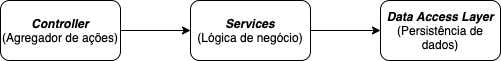
\includegraphics[width=0.85\textwidth]{controllerservicedal}
      \caption{Conceitos utilizados no servidor}
  \label{fig:controllerservicedal_s}
\end{figure}


No servidor, foram utilizados métodos assíncronos, recorrendo à ativação e configuração do processo assíncrono \textit{Spring}, que permite detetar as operações assíncronas utilizando a anotação @Async. Na configuração do processo, é criado um executor de tarefas, definindo o número de \textit{threads} sempre disponíveis para receber tarefas, o número máximo de \textit{threads} que podem ser criadas para processamento, assim como o máximo de tarefas que podem estar numa fila à espera para serem processadas. Quando o contexto do \textit{Spring} é inicializado, marca os métodos que têm a anotação @Async como assíncronos, o que permite utilizar um gestor de tarefas quando um método marcado é invocado, para ser executado numa nova \textit{thread} em pararelo. Com isso é possível ter respostas mais rápidas ao cliente, realizando o processamento de outras ações mais complexas em \textit{threads} diferentes. O cálculo da previsão de tempo de espera e o envio de notificações, são realizadas em processos assíncronos visto que são mais demorados, pela necessidade de obtenção de mais dados e consequente processamento, e por ser necessário no caso do envio de notificações, a comunicação com o serviço externo \textit{\acrshort{fcm}}.

Na camada de acesso a dados, foi utilizada uma cache simples o que permite obter dados que não são alterados constantemente (e.g. sessão) de forma mais rápida, sem a necessidade de realizar um pedido à base de dados. Tendo em conta que se está no contexto de uma prova de conceito, não é realizada a implementação de um mecanismo que permite inserir dados com um tempo de vida e remove-los quando o tempo expira. 

A componente servidor, à medida que foi desenvolvida, foi-se realizando o \textbf{\textit{deployment}} de versões estáveis para a \textbf{\textit{cloud}}. Para hospedagem, foi utilizada a plataforma Heroku. O \textit{deployment} é realizado de forma automática, recorrendo a \textit{pipelines} presentes no repositório git do projeto, tendo sido necessário realizar configurações do lado do Heroku e do Bitbucket (onde se encontra o repositório do projeto) e a criação de um ficheiro bitbucket-pipelines.yml. No ficheiro estão indicados os passos a serem dados quando é detetado que houve \textit{commits} no \textit{branch master} (versão estável), sendo elas, a criação de um artefato que contém o projeto em \textit{Spring Boot} e o envio para o Heroku. A plataforma de hospedagem ao receber o artefacto faz o \textit{build} do projeto e em caso de sucesso, ocorre o \textit{deploy}, ficando automaticamente disponível para utilização por parte dos utilizadores. O servidor de base de dados está também hospedado na plataforma Heroku.

A \textbf{Aplicação Móvel} cliente do sistema implementada em Android, utilizando a arquitetura recomendada para desenvolvimento Android \cite{androidrecomm}, baseada no padrão \textit{\acrfull{mvvm}} \cite{mvvm}, fornece ao utilizador uma interface que permite a realização da autenticação no sistema, sendo apresentado um conjunto de serviços, em caso de sucesso. O utilizador pode escolher o serviço pretendido, sendo apresentado todos os postos de serviço disponibilizados pela entidade institucional. Em cada posto de serviço, é possível observar um conjunto de filas, que permite ao utilizador a visualização do estado das filas assim como o tempo de espera previsto. O estado das filas é atualizado em tempo real, ao receber \textit{push notifications} com informação atualizada. Isto é possível com uma subscrição implícita sobre o posto por parte da aplicação. Ao selecionar uma fila, o utilizador pode optar por retirar uma senha. Com a obtenção de uma senha, a aplicação recorre a serviços \textit{Android} de forma a disponibilizar ao utilizador uma notificação que apresenta o estado da fila e do tempo de espera. À medida que a aplicação vai recebendo atualizações do servidor em combinação com \acrshort{fcm}, o serviço recebe eventos de forma a manipular a notificação com os dados corretos.

A aplicação que serve de \textbf{simulador de serviço}, desenvolvido em Flutter Web, utiliza o mesmo padrão (\acrshort{mvvm}) que a aplicação móvel, tendo três modos de utilização, sendo eles administrador, administrador de serviço e servidor de serviço. Cada modo, depende do tipo de utilizador que realiza a autenticação, com o simulador a receber informação suficiente de forma a encaminhar o utilizador. Os modos estão separados em módulos no projeto, onde cada um contêm as interfaces gráficas e gestores de estados específicos, permitindo uma navegação diferente para cada tipo de utilizador.  

\subsection{Funcionalidades} 
Nesta secção é descrito as funcionalidades base do sistema.

\subsubsection{Registo}
O registo de utilizadores é diferente para cada tipo de utilizador do sistema, sendo que o administrador é que faz a gestão dos administradores e servidores de serviços, não tendo a possibilidade de realizar um registo autónomo. No entanto, o utilizador cliente da aplicação móvel pode realizar o registo, utilizando a aplicação, fornecendo os dados necessários para o registo com sucesso. Por este projeto ser uma prova de conceito, a ação é realizada de forma simples, sem a necessidade de confirmação por parte do cliente (e.g. confirmação por email) e sem aplicar o \acrfull{rgpd} \cite{rgpd}. Visto que existe recolha e tratamento de dados do utilizador, num cenário real seria necessário aplicar o \acrshort{rgpd} no projeto.

\subsubsection{Autenticação e Autorização} 
A autenticação e autorização é realizada pelo próprio servidor sem a utilização de protocolos e servidores de autenticação externos, o que permite ter um sistema com maior autonomia. O utilizador ao estar autenticado, utiliza um \textit{token} de acesso, gerado e fornecido pelo sistema, para realizar as operações pelas quais está autorizado. De forma a garantir maior flexibilidade do sistema, esta componente integrada com outros serviços de identificação de utilizadores, permitindo assim acessos sem a necessidade de realizar um novo registo. A autorização é realizada recorrendo às entidades \textit{User\_Service}, \textit{User\_Post\_Office} e \textit{Path\_Control\_Access}.

No JSON abaixo é possível ver a estrutura enviada pelo servidor para as aplicações clientes no momento da atualização. O nome é utilizado meramente para dar as boas vindas ao utilizador e indicar as iniciais quando o utilizador entra no menu da aplicação móvel. A indicação do \textit{role}, permite identificar o tipo de utilizador e enviar para o módulo correto no simulador de serviço. O \textit{token}, será utilizado em todas as operações que requerem o utilizador autenticado, sendo utilizado também para validar se o utilizador está autorizado para realizar a operação. O \textit{userId} e \textit{role} são utilizados apenas para simplificar e permitir operações mais rápidas, sem a necessidade de haver introspeção e pedidos extras no servidor para obtenção da informação para realização de ações.

\begin{lstlisting}[language=json,firstnumber=1]
{
    "class": [
        "session"
    ],
    "properties": {
        "name": "Ronilton Neves",
        "role": "ADMIN",
        "token": "f60cc0c2-a975-4c4b-8de1-c8e6f05754a5",
        "userId": 1
    }
}
\end{lstlisting}

\subsubsection{Visualização de Estado e Obtenção de Senhas} 
O utilizador após a autenticação com sucesso consegue ver os serviços e os postos de serviços disponíveis, assim como as filas de cada posto. Ao entrar num posto de serviço, é realizado uma subscrição implícita de forma automática, o que representa uma declaração de interesse sobre os estados das filas do posto de serviço. Ao deixar de observar a informação de um posto a subscrição é retirada de forma automática. Durante o período em que o utilizador tem a informação disponível, é atualizado das alterações em tempo real. 

O utilizador tem a opção para escolher uma fila do serviço e requisitar uma senha, ficando subscrito de forma explícita, com a aplicação móvel a lançar um serviço em primeiro plano que vai apresentando o estado da fila e o tempo de espera previsto, permitindo ao utilizador fechar a aplicação, e continuar a receber as atualizações até ser atendido.

No objeto JSON abaixo é possível observar um exemplo da estrutura que contém o estado das filas de espera de um posto de serviço. Neste exemplo é possível observar que o posto de serviço, tem duas filas (A e B), tendo o valor de atendimento presente na propriedade \textit{attendedNumber}, a última senha retirada \textit{stateNumber}, com \textit{name}, \textit{letter} e \textit{queueId} sendo as informações da fila e por fim a previsão do tempo de espera na propriedade \textit{forecast}.

\begin{lstlisting}[language=json,firstnumber=1]
{
    "class": [
        "collection",
        "queueStates"
    ],
    "properties": {
        "queueStates": [
            {
                "class": [
                    "queueState"
                ],
                "properties": {
                    "stateNumber": 13,
                    "name": "Queue A",
                    "letter": "A",
                    "queueId": 4,
                    "attendedNumber": 5,
                    "forecast": 134
                }
            },
            {
                "class": [
                    "queueState"
                ],
                "properties": {
                    "stateNumber": 5,
                    "name": "Queue B",
                    "letter": "B",
                    "queueId": 5,
                    "attendedNumber": 5,
                    "forecast": 0
                }
            }
        ]
    }
}
\end{lstlisting}

\subsubsection{Atualizações em tempo real} 
Nesta secção está descrito o processo que permite a atualização em tempo real do estado das senhas. Na \figurename~\ref{fig:live_update} é possível observar o esquema de atualização. 

\begin{figure}[ht]
	\centering
	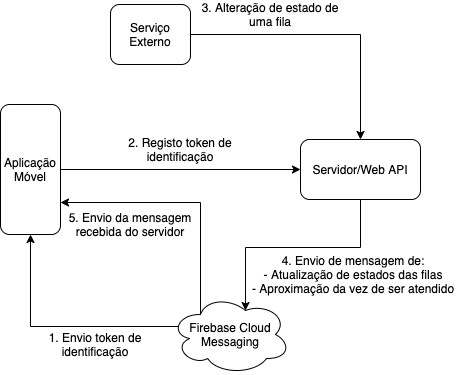
\includegraphics[width=0.85\textwidth]{fcm}
	  \caption{Esquema da atualização em tempo real}
  \label{fig:live_update}
\end{figure}

Da primeira vez que o utilizador inicia a aplicação móvel, um \textit{token} de identificação que associa um dispositivo à aplicação é gerado pelo serviço de \acrshort{fcm}, sendo enviado ao servidor quando o utilizador realiza a primeira autenticação, de modo a permitir enviar notificações/mensagens para os utilizadores corretos. No passo 1 e 2 da \figurename~\ref{fig:live_update} é possível verificar o registo do \textit{token}. O processo de geração e consequente registo, pode ser repetido diversas vezes, visto que existe um mecanismo de rotação de \textit{tokens}, sendo atualizado pelo \acrshort{fcm} e enviado para a aplicação móvel. 

Com o registo do \textit{token} e as subscrições sobre serviços e senhas, o utilizador fica habilitado a receber atualizações em tempo real, com o desencadeamento dos passos 3, 4 e 5. Num serviço externo ao sistema, ao ser alterado o estado da fila, este tem que informar o sistema, permitindo a este anunciar aos interessados o evento. O servidor, de acordo com a informação recebida, realiza um processamento de forma a identificar quem recebe a atualização do estado e quem recebe informação sobre aproximação da vez de ser atendido. Com o processamento completo, os dados são enviados para o \acrshort{fcm}, com a identificação (\textit{token}) de cada utilizador, permitindo o \acrshort{fcm} a entrega ao destinatário correto da informação recebida.

No JSON abaixo é possível verificar um exemplo do formato de dados que é enviado a um utilizador que tenha uma subscrição sobre uma fila. 

\begin{lstlisting}[language=json,firstnumber=1]
{
	"type": "ticket_for_list",
	"queueId" : 1,
	"letter" : "A",
	"stateNumber" : 5,
	"attendedNumber" : 2,
	"name": "Queue A",
	"forecast" : 120
}
\end{lstlisting}

A aplicação cliente pode receber diferentes formatos de mensagens do \acrshort{fcm}, sendo responsável por realizar o processamento adequado de forma a apresentar corretamente os dados ao utilizador.

\newpage

\subsection{Modelo de Dados}
O modelo de dados utilizado pelo sistema, é baseado no diagrama Entidade Associação (\acrshort{ea}) apresentado na \figurename~\ref{fig:model}. De forma a garantir a persistência dos dados utilizados, este utiliza um servidor de base de dados PostgreSQL.

\begin{figure}[ht]
    \centering
    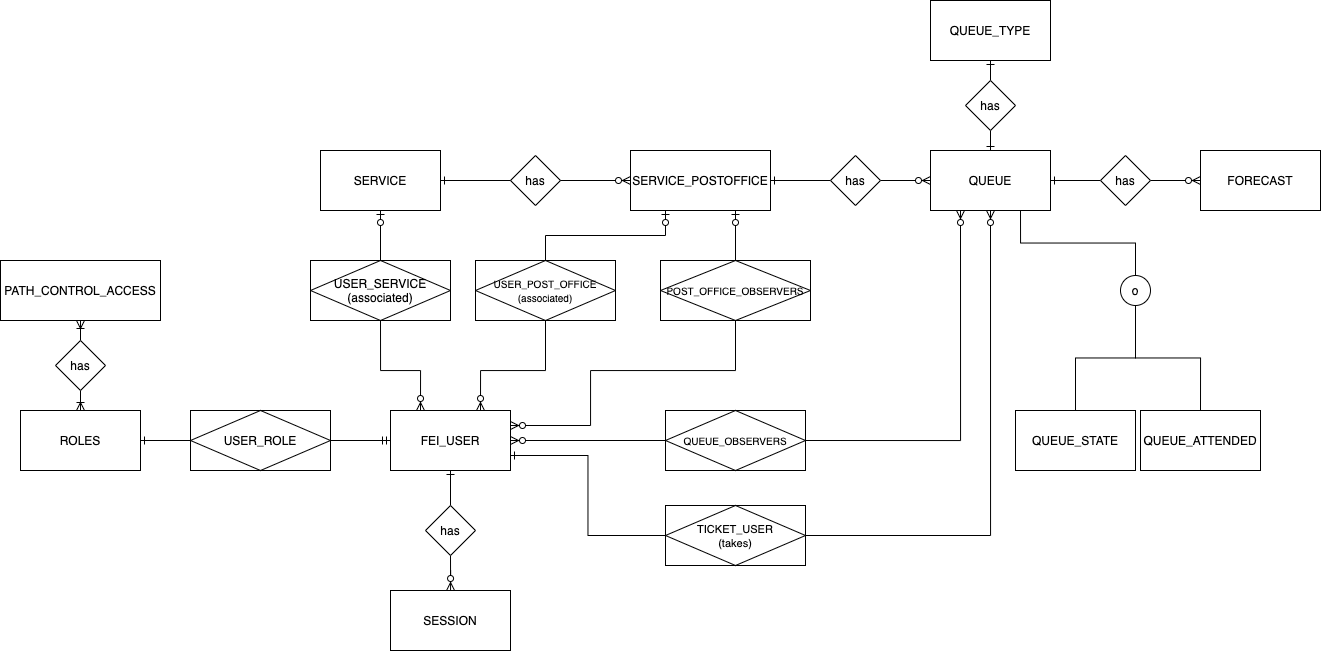
\includegraphics[width=1\textwidth]{ea_model}
      \caption{Diagrama EA do modelo de dados}
  \label{fig:model}
\end{figure}

\textbf{Fei\_user}(\textit{\underline{id}, username, name, nif, password, salt, fcm\_token, phone, email, state}) - Entidade que contém os dados dos utilizadores do sistema.

\textbf{Service}(\textit{\underline{id}, name, description, state}) - Entidade que tem a informação dos serviços integrados no sistema.

\textbf{Service\_Postoffice}(\textit{\underline{id}, latitude, longitude, description, serviceId[FK], address, state}) - Tem informação de cada posto pertencente a um determinado serviço.

\textbf{Queue\_Type}(\textit{\underline{id}, description, state}) - Tem a informação sobre os tipos de fila.

\textbf{Queue}(\textit{\underline{id}, activeServers, letter, name, description, type, maxAvailable, servicePostOfficeId[FK], tolerance, state}) - Tem a informação relaciona com as filas de cada posto de serviço.

\textbf{Queue\_State}(\textit{\underline{id}, number, letter, queueId[FK]}) - Tem a informação do estado atual das filas.

\textbf{Queue\_Attended}(\textit{\underline{id}, number, letter, queueId[FK]}) - Tem a informação do estado de atendimento das filas por parte dos servidores.

\textbf{Ticket\_User}(\textit{\underline{id}, queueId[FK], number, userId[FK], createdAt, attended, duration, state, canceled, forecast, updatedAt}) - Esta entidade associação, é utilizada quando um utilizador obtém a senha de um determinado serviço. 

\textbf{Session}(\textit{\underline{id}, userId[FK], token, createdAt}) - Entidade responsável por armazenar as sessões dos utilizadores logados.

\textbf{Forecast}(\textit{\underline{id}, queueId[FK], alpha, flimit, forecast}) - Entidade que contêm a informação que deve ser aplicada a cada fila de espera para obtenção da previsão.

\textbf{Roles}(\textit{\underline{id}, role}) - Tem as funções dos utilizadores do sistema.

\textbf{User\_Role}(\textit{\underline{userId}, role}) - Contêm a associação entre utilizador e função.

\textbf{Queue\_Observers}(\textit{\underline{id}, queueId[FK], userId[FK]}) - Entidade associação responsável por armazenar os observadores de cada fila.

\textbf{Post\_Office\_Observers}(\textit{\underline{id}, postId[FK], userId[FK]}) - Entidade associação responsável por armazenar os observadores de cada posto de serviço.

\textbf{User\_Service}(\textit{\underline{userId}, serviceId[FK]}) - Tem a informação de que serviços é que um utilizador pode aceder. 

\textbf{User\_Post\_Office}(\textit{\underline{userId}, servicePostOfficeId[FK]}) - Tem a informação de que postos de serviço é que um utilizador tem acesso.

\textbf{Path\_Control\_Access}(\textit{\underline{id}, method, regex, roles}) - É a entidade onde está definido as regras de acesso de cada função no sistema.

Em algumas entidades do modelo, é possível verificar o atributo \textit{state} (tipo \textit{bit}) que serve para representar se um registo está válido ou não, permitindo assim manter histórico sem a necessidade da criação de novas entidades. Com isso, ao ocorrer uma tentativa de eliminação de um recurso, o sistema apenas faz a atualização do atributo \textit{state} para zero (0) e o recurso deixa de estar visível.

De forma a auxiliar na inserção e atualização de dados, foram implementadas algumas funções, \textit{procedures} e \textit{triggers}. Um dos \textit{procedures} existentes é o \textit{SetUser\_Ticket\_Attended} que é responsável por indicar que um cliente já foi atendido, realizando também o cálculo do tempo de atendimento, que é utilizado posteriormente para o cálculo de previsão de tempo da fila. As funções \textit{Create\_Queue\_Tables} e \textit{Update\_Queue\_Tables} são utilizadas por \textit{triggers} de forma a inserir e atualizar as entidades \textit{Queue\_State} e \textit{Queue\_Attended} quando existe uma inserção ou atualização na entidade \textit{Queue}. Uma outra função importante é o \textit{Get\_Next\_In\_Line} que permite obter o próximo cliente na fila, para que este seja notificado que a vez de ser atendido se aproxima. \\

